\section{The ACE Service}\label{sec:the-ace-service}

ACE or the Ambulatory Care Experience is a service that delivers paediatric urgent care in the Bradford community.
As part of Bradford Teaching Hospitals Foundation Trust's ``virtual wards'' strategy, ACE is intended to improve patient outcomes and deliver value for money \cite{kingsfund}.
Indeed, the Care Quality Commission reports have singled out the ACE service as ``outstanding practice'' and ``make[ing] best use of clinical resources'' \cite{cqc}.
The service has also been awarded a Health Services Journal ``Improvement in Emergency and Urgent Care'' award \cite{hsj_award}.

The primary aim of the ACE service is to avoid hospitalisation.
Children who require ongoing specialist assessment, treatment and monitoring can be looked after by ACE from the comfort of their own homes, under the care of a nurse and consultant paediatrician.
The team support and monitor the effectiveness of treatments, taking care to note any deterioration in the patient that may indicate the need for hospital treatment.
\Cref{fig:ace-pathway} details the ACE treatment pathway for CYP with ``wheeze/asthma''.
This approach avoids the traditional pathway of hospitalisation, assessment, observation and discharge without need for further treatment, that is often seen in paediatric urgent care.

\begin{figure}[H]
    \centering
    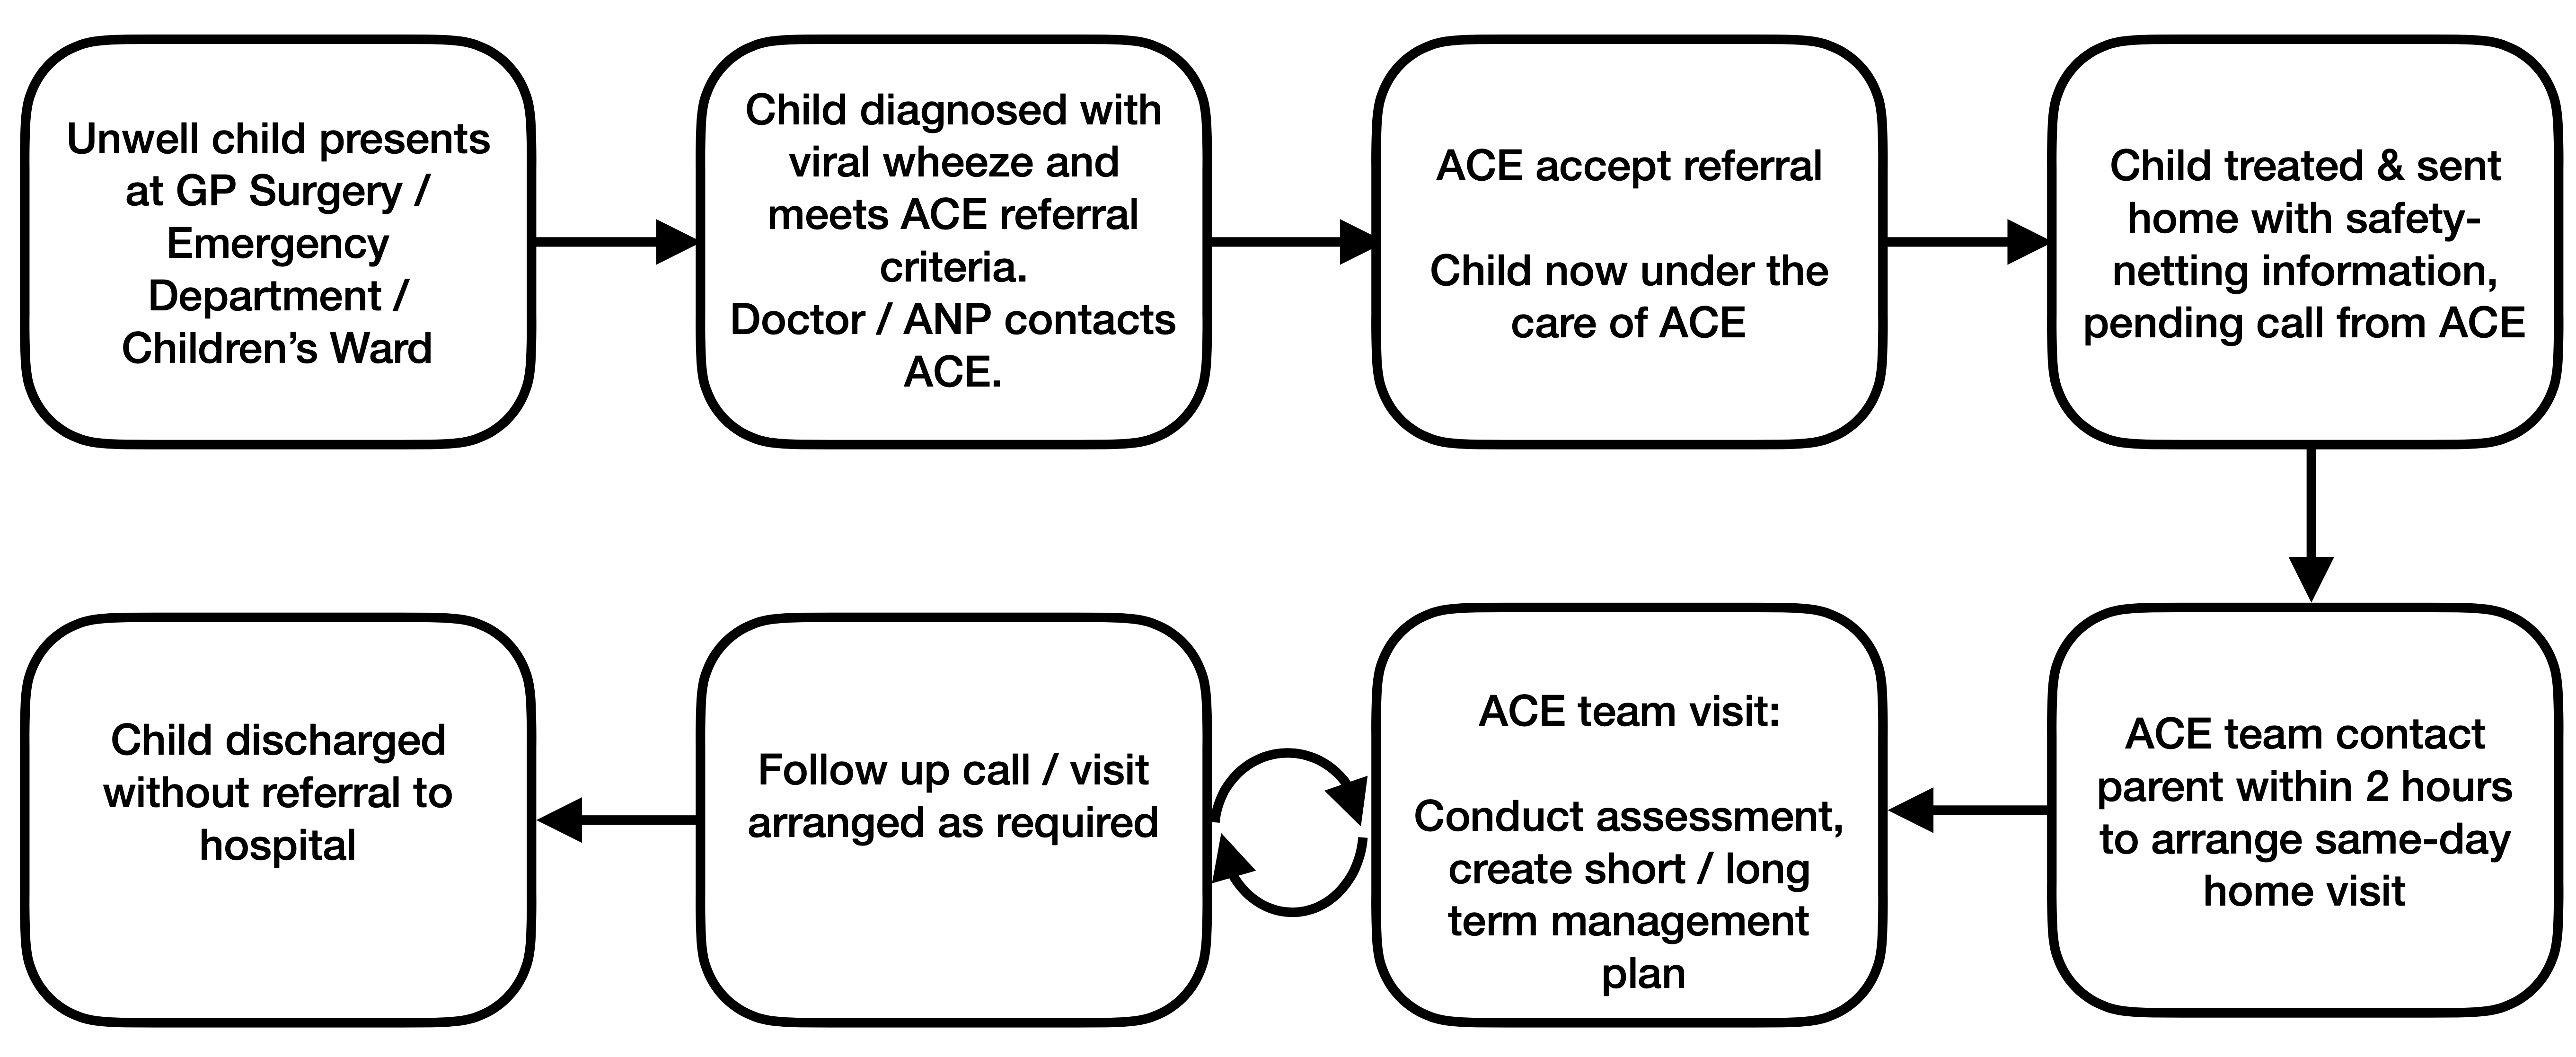
\includegraphics[width=1\textwidth]{ace_pathway}
    \caption[ACE asthma/wheeze referral pathway]{The referral pathway for an ACE patient referred with asthma/wheeze and successfully discharged without hospital referral}
    \label{fig:ace-pathway}
\end{figure}

Key to the success of ACE is deciding which of the referred patients are of ``mild to moderate concern''.
The service can only reduce hospitalisations if their patients are being discharged without later being hospitalised.
ACE define a set of referral criteria that indicate suitability for home treatment.
Examples of these criteria for the viral wheeze / asthma pathway can be seen in \Cref{fig:referral-criteria}.
Patients are accepted for community treatment if the referrer and ACE team judge that this is appropriate (even if the clinical parameters fall outside the set referral criteria).
These referral decisions contribute to the successful discharge of 84\% of patients, based on current data.

The principle need for urgent care in this setting is observation and monitoring for deterioration.
Thus, the expectation is that some patients will inevitably require later hospital treatment.
Nonetheless, the aim of ACE is to ensure the number of patients hospitalised under their care is as low as possible.

\begin{figure}[h]
    \centering
    \begin{tabular}{ P{41mm} P{20mm} P{20mm} }
        \toprule
        \textbf{Oxygen saturations in air} & \multicolumn{2}{l}{\textless  94\% }\\[0.7cm]
        \textbf{Heart Rate} & \textbf{Age:} & \textbf{Value:} \\
        \textbf{(beats per minute)} & 2--5 years & 95--140 \\
        & 5--12 years & 80--120 \\
        & \textgreater 12 years & 60--100 \\[0.2cm]
        \textbf{Respiratory Rate} & \textbf{Age:} & \textbf{Value:} \\
        \textbf{(breaths per minute)} & 2--5 months & 25--30 \\
        & 5--12 years & 20--25 \\
        & \textgreater 12 years & 15--20 \\[0.2cm]
        \textbf{Auscultation} & \multicolumn{2}{l}{Good air entry with some wheeze}\\[0.2cm]
        \textbf{Speech} & \multicolumn{2}{l}{Able to complete sentences}\\[0.2cm]
        \textbf{Work of breathing} & \multicolumn{2}{l}{Minimal/no recessions}\\[0.2cm]
        \textbf{Conscious level} & \multicolumn{2}{l}{normal}\\[0.2cm]
        \toprule
    \end{tabular}
\caption[ACE referral criteria]{The ACE referral criteria. A set of clinical characteristics that indicate a patient is of mild to moderate concern and is suitable for treatment within ACE. Note: Patients can be accepted for treatment even if their observations fall outside these criteria.}
\label{fig:referral-criteria}
\end{figure}

\section{Predicting ACE Treatment Outcomes}\label{sec:predicting-ace-treatment-outcomes}

ACE clinicians have long been preoccupied with the characteristics that make a paediatric urgent care patient suitable for treatment at home.
Having collected 3 years of referral data, they hypothesised that modern machine learning techniques could use this data to predict treatment outcomes within the service.
This project aimed to test that hypothesis.

We aimed to answer the following three questions:

\begin{enumerate}
    \item Can machine learning classification models use ACE referral data to accurately predict which patients required hospital treatment?

    Machine learning has already shown great potential in a range of clinical settings \cite{topol_2019}. Repositories of high quality labelled data found in the healthcare setting offer an abundance prospective applications of machine learning. Among these applications are many successful examples of risk modelling \cite{golas_2018} \cite{rahimian_2018} \cite{desautels_2016}. With their own labelled referral records, the ACE team hypothesise that a similar approach might be applied to predict the risk of hospitalisation for patients referred to the ACE service.

    \item Are there predictors of hospital referral that can be identified from the ACE referral data?

    An important aspect of predictive modelling, especially so in the healthcare setting, is \textit{why} a prediction was made. The ACE team are particularly interested the \textit{predictors} of hospitalisation risk, alongside the \textit{predictions} themselves -  which features increase a patient's risk of a hospital referral, or indicate that a patient is more suitable for home treatment? Many predictive modelling approaches are capable of offering such insights, be they ``explainable'' predictive modelling techniques, or post-hoc explainability methods - we aim to use such methods to identify predictors of hospitalisation.

    \item Can we quantify our uncertainty / certainty in the findings from questions 1 and 2?

    The size and scope of the ACE service is such that training data is scarce. Any inferences drawn from this data will be supported by very few real examples. As such, it will be as important to quantify what \textit{can't} be said based on the referral data as what \textit{can}. Under what circumstances can we be confident of an outcome or of the effect of a given feature, and when are we less certain? This work aims to test methods that can predict not only the chance of a given outcome but also the error, or anticipated range of resonable values, for this prediction.

\end{enumerate}
